%---------------------------------------------------------------------------%
%-                                                                         -%
%-                           LaTeX Template                                -%
%-                                                                         -%
%---------------------------------------------------------------------------%
%- Copyright (C) Huangrui Mo <huangrui.mo@gmail.com> 
%- This is free software: you can redistribute it and/or modify it
%- under the terms of the GNU General Public License as published by
%- the Free Software Foundation, either version 3 of the License, or
%- (at your option) any later version.
%---------------------------------------------------------------------------%
%->> Document class declaration
%---------------------------------------------------------------------------%
\documentclass[twoside]{Style/ucasthesis}%
%- Multiple optional arguments:
%- [<oneside|twoside|print>]% oneside eprint, twoside eprint, or paper print
%- [fontset=<adobe|none|...>]% specify font set instead of automatic detection
%- [scheme=plain]% thesis writing of international students
%- [draftversion]% show draft version information
%- [standard options for ctex book class: draft|paper size|font size|...]%
%---------------------------------------------------------------------------%
%->> Document settings
%---------------------------------------------------------------------------%
\usepackage[super,list]{Style/artratex}% document settings
%- usage: \usepackage[option1,option2,...,optionN]{artratex}
%- Multiple optional arguments:
%- [bibtex|biber]% set bibliography processor and package
%- [<numbers|super|authoryear|alpha>]% set citation and reference style
%- <numbers>: textual: Jones [1]; parenthetical: [1]
%- <super>: textual: Jones superscript [1]; parenthetical: superscript [1]
%- <authoryear>: textual: Jones (1995); parenthetical: (Jones, 1995)
%- <alpha>: textual: not available; parenthetical: [Jon95]
%- [geometry]% reconfigure page layout via geometry package
%- [lscape]% provide landscape layout environment
%- [xhf]% disable header and footer via fancyhdr package
%- [color]% provide color support via xcolor package
%- [background]% enable page background
%- [tikz]% provide complex diagrams via tikz package
%- [table]% provide complex tables via ctable package
%- [list]% provide enhanced list environments for algorithm and coding
%- [math]% enable some extra math packages
%- [xlink]% disable link colors
\usepackage{Style/artracom}% user defined commands

\usepackage{amsmath}

\usepackage{ulem}

\usepackage{graphicx}

\usepackage{animate}
%---------------------------------------------------------------------------%
%->> Document inclusion
%---------------------------------------------------------------------------%
%\includeonly{Tex/Chap_1,...,Tex/Chap_N}% selected files compilation
%---------------------------------------------------------------------------%
%->> Document content
%---------------------------------------------------------------------------%
%-
%-> Titlepage information
%-
%---------------------------------------------------------------------------%
%->> Titlepage information
%---------------------------------------------------------------------------%
%-
%-> 中文封面信息
%-
\confidential{}% 密级:只有涉密论文才填写
\schoollogo[scale=0.045]{leeds_logo}% 校徽
\title{Deep Learning 学习笔记}% 论文中文题目
\author{莫晃锐}% 论文作者
\advisor{刘青泉~研究员~中国科学院力学研究所\\}% 指导教师:姓名 专业技术职务 工作单位
%\advisor{指导教师一\\指导教师二\\指导教师三}% 多行指导教师示例
\degree{学士}% 学位:学士、硕士、博士
\degreetype{理学}% 学位类别:理学、工学、工程、医学等
\major{流体力学}% 二级学科专业名称
\institute{中国科学院力学研究所}% 院系名称
%\institute{中国科学院力学研究所\\流固耦合实验室}% 多行院系名称示例
\date{2014~年~6~月}% 毕业日期:夏季为6月、冬季为12月
%-
%-> 英文封面信息
%-
\TITLE{\LaTeX{} Thesis Template\\ of \\ The University of Chinese Academy of Sciences {$~^{\pi}\pi^{\pi}$}}% 论文英文题目
\AUTHOR{Mo Huangrui}% 论文作者
\ADVISOR{Supervisor: Professor Liu Qingquan}% 指导教师
\DEGREE{Master}% 学位:Bachelor, Master, Doctor, Postdoctor。封面据英文学位名称自动切换,需确保拼写准确
\DEGREETYPE{Natural Science}% 学位类别:Philosophy, Natural Science, Engineering, Economics, Agriculture 等
\MAJOR{Fluid Mechanics}% 二级学科专业名称
\INSTITUTE{Institute of Mechanics, Chinese Academy of Sciences}% 院系名称
\DATE{June, 2014}% 毕业日期:夏季为June、冬季为December
%---------------------------------------------------------------------------%
%
\begin{document}
%-
%-> Frontmatter: title page, abstract, content list, symbol list, preface
%-
\frontmatter% initialize the environment
%---------------------------------------------------------------------------%
%->> Frontmatter
%---------------------------------------------------------------------------%
%-
%-> 生成封面
%-
%\maketitle% 生成中文封面
%\MAKETITLE% 生成英文封面
%-
%-> 作者声明
%-
%\makedeclaration% 生成声明页
%-
%-> 中文摘要
%-
\intobmk\chapter*{摘\quad 要}% 显示在书签但不显示在目录
\setcounter{page}{1}% 开始页码
\pagenumbering{Roman}% 页码符号

本文是我在学习深度学习有关知识时的笔记~。

\keywords{深度学习}% 中文关键词
%-
%-> 英文摘要
%-
\intobmk\chapter*{Abstract}% 显示在书签但不显示在目录

This article is my notes while learning deep learning~.

\KEYWORDS{deep learning}% 英文关键词
%---------------------------------------------------------------------------%
% title page, abstract
{% content list region
\linespread{1.2}% local line space
\intobmk*{\cleardoublepage}{\contentsname}% add link to bookmark
\tableofcontents% content catalog
\intobmk*{\cleardoublepage}{\listfigurename}% add link to bookmark
\listoffigures% figure catalog
\intobmk*{\cleardoublepage}{\listtablename}% add link to bookmark
\listoftables% table catalog
}
\intobmk\chapter*{符号列表}% 显示在书签但不显示在目录

%\section*{字符}
%\nomenclatureitem[\textbf{Unit}]{\textbf{Symbol}}{\textbf{Description}}
%\nomenclatureitem[$\Unit{m^{2} \cdot s^{-2} \cdot K^{-1}}$]{$R$}{the gas constant}
%\nomenclatureitem[$\Unit{m^{2} \cdot s^{-2} \cdot K^{-1}}$]{$C_v$}{specific heat capacity at constant volume}
%\nomenclatureitem[$\Unit{m^{2} \cdot s^{-2} \cdot K^{-1}}$]{$C_p$}{specific heat capacity at constant pressure}
%\nomenclatureitem[$\Unit{m^{2} \cdot s^{-2}}$]{$E$}{specific total energy}
%\nomenclatureitem[$\Unit{m^{2} \cdot s^{-2}}$]{$e$}{specific internal energy}
%\nomenclatureitem[$\Unit{m^{2} \cdot s^{-2}}$]{$h_T$}{specific total enthalpy}
%\nomenclatureitem[$\Unit{m^{2} \cdot s^{-2}}$]{$h$}{specific enthalpy}
%\nomenclatureitem[$\Unit{kg \cdot m \cdot s^{-3} \cdot K^{-1}}$]{$k$}{thermal conductivity}
%\nomenclatureitem[$\Unit{kg \cdot m^{-1} \cdot s^{-2}}$]{$S_{ij}$}{deviatoric stress tensor}
%\nomenclatureitem[$\Unit{kg \cdot m^{-1} \cdot s^{-2}}$]{$\tau_{ij}$}{viscous stress tensor}
%\nomenclatureitem[$\Unit{1}$]{$\delta_{ij}$}{Kronecker tensor}
%\nomenclatureitem[$\Unit{1}$]{$I_{ij}$}{identity tensor}

\section*{算子}
\nomenclatureitem{\textbf{Symbol}}{\textbf{Description}}
\nomenclatureitem{$\int$}{Indefinite integral}
\nomenclatureitem{$\sum$}{Sum}
\nomenclatureitem{$*$}{Convolution}

\section*{缩写}
\nomenclatureitem{CNN}{Convolutional Neural Network}

% symbol list, preface content
%-
%-> Mainmatter
%-
\mainmatter% initialize the environment
%---------------------------------------------------------------------------%
%->> Main content
%---------------------------------------------------------------------------%
\chapter{卷积层}

\section{卷积层的特点}
	
	全连接层存在什么问题呢?那就是数据的形状被“忽视”了。比如,输入数据是图像时,图像通常是高、长、通道方向上的3维形状。但是,向全连接层输入时,需要将3维数据拉平为1维数据。全连接层会忽视形状,将全部的输入数据作为相同的神经元(同一维度的神经元)处理,所以无法利用与形状相关的信息。
	
	而卷积层可以保持形状不变。当输入数据是图像时,卷积层会以3维数据的形式接收输入数据,并同样以3维数据的形式输出至下一层。因此在CNN中,可以(有可能)正确理解图像等具有形状的数据。
	
	CNN中,有时将卷积层的输入输出数据称为特征图(feature map)。其中,卷积层的输入数据称为输入特征图(input feature map),输出数据称为输出特征图(output feature map)\cite{RN1}。

\section{卷积运算}
	
	卷积层进行的处理就是卷积运算。卷积运算相当于图像处理中的“滤波器运算”。
	
	“卷积是一种特殊的加权求和”。
	\subsection{一维离散卷积}
		\subsubsection{引入——多项式乘法}
		
		设多项式:
		\begin{equation}
			\label{eq:1}
			P\left(x\right) = a_n x^n + a_{n-1} x^{n+1} + \cdots + a_1 x + a_0
		\end{equation}
	
		\begin{equation}
			\label{eq:2}
			Q\left(x\right) = b_m x^m + b_{m-1} b^{m+1} + \cdots + b_1 x + b_0
		\end{equation}
	
		那么,
		
		\begin{equation}
			\begin{aligned}
			R\left(x\right) &= P\left(x\right) \times Q\left(x\right) \\
			& = \left( \sum_{i=0}^{n} a_i x^i\right) \cdot \left( \sum_{i=0}^{m} b_i x^i\right) \\
			& = \sum_{i=0}^{m+n} c_i x^i \\
			where, \quad c_i & = \sum_k a_k b_{i-k}
			\end{aligned}
		\end{equation}
		
		接下来,我们以 $P\left(x\right) = x^4 -x^3 +2x -4$, $Q\left(x\right) = x^2 -2x +2$ 为例。其计算结果为:$$R\left(x\right) = x^6 -3x^5 + 4x^4 -8x^2+12x-8$$
		
		其乘法的直观表示如图所示:
		\begin{figure}[!htbp]
			\centering
			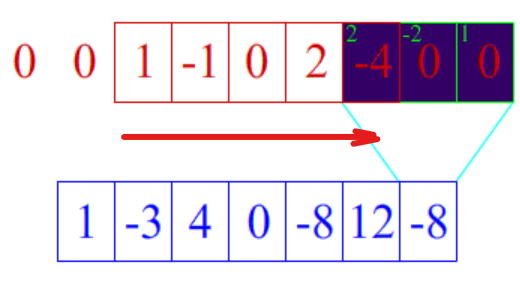
\includegraphics[width=0.50\textwidth]{conv_1}
			\caption{乘法的直观表示}
			\label{fig:1}
		\end{figure}
		
		在图\ref{fig:1}中,需要注意$Q\left(x\right)$的系数是反转哒。
		
		\subsubsection{一维离散卷积的定义}
		\begin{definition}
			如果$\left\{a_n\right\}$ $\left\{b_m\right\}$ 是两个数列, 那么二者的卷积为:
			$$c_i = \left(a * b\right) _i = \sum_k a_k b_{i-k}$$
			其中,$\left\{a_n\right\}$ 是被卷积数列, $\left\{b_m\right\}$是卷积核。
		\end{definition}
	
		在上面的例子中,如果下标不合法,则用0来代替——这是完全补0的卷积,也叫\textbf{Full卷积}。类似的,我们也可以定义如图\ref{fig:2}所示的合法卷积,也叫\textbf{Valid卷积}。
		
		\begin{figure}[!htbp]
			\centering
			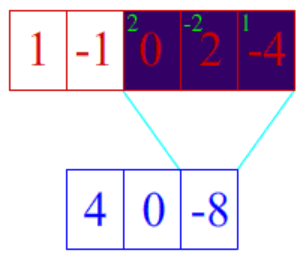
\includegraphics[width=0.30\textwidth]{conv_2}
			\caption{Valid Convolution}
			\label{fig:2}
		\end{figure}
	
		同样的,我们也可以定义\textbf{Same卷积}——卷积后的数列长度和被卷积数列一样长。具体操作仅仅比Full卷积左右各少补一半的0就可以了。
		
		在此基础上,卷积核并不一定是在被卷积数列上一格一格地滑动,可以两格两格,甚至半格半格地滑动,由此派生出无数种可能\cite{RN2}。
	\subsection{一维连续卷积}
		
		上文中涉及到的都是离散的数列,如果改为连续函数$f\left(x\right)$ 与 $g\left(x\right)$ 的卷积,那么:
        \begin{equation}
            h\left(x\right) = \left( f*g \right) \left(x\right) = \int {f\left(\tau \right) g\left(x-\tau \right)d\tau}
            \label{eq:3}
        \end{equation}
        下面我们举一个具体的例子。
        
        假设你是一个算法工程师,过着996的死亡生活,每天除了调参就是调参。你每天工作效率关于时间$t$的函数为$f\left(t\right)$ (显然,如果你准时上班,正点下班,那么$f\left(t\right) $在 $\left[0,9\right) \bigcup \left[ 21,24 \right)$ 上是没有定义的)。并且工作成果的产出关于时间$t$的函数为$g\left(x\right)$,那么你忙活一天,给团队获得的实际收益则是: 
        $$ h\left(24\right) = \int_{9}^{21} {f\left(\tau \right) g\left(24-\tau \right)d\tau} $$
    \subsection{二维离散卷积}
        上述的卷积都是一维的卷积核在一维的被卷积张量上滑动。如果被卷积张量和卷积核是二维、三维,甚至四维及以上,我们同样也可以有相同的定义——向这些维度分别滑动,分别做卷积,最后求和即可。
        \subsubsection{二维离散卷积}
        
        \begin{figure}[!htbp]
            \centering
            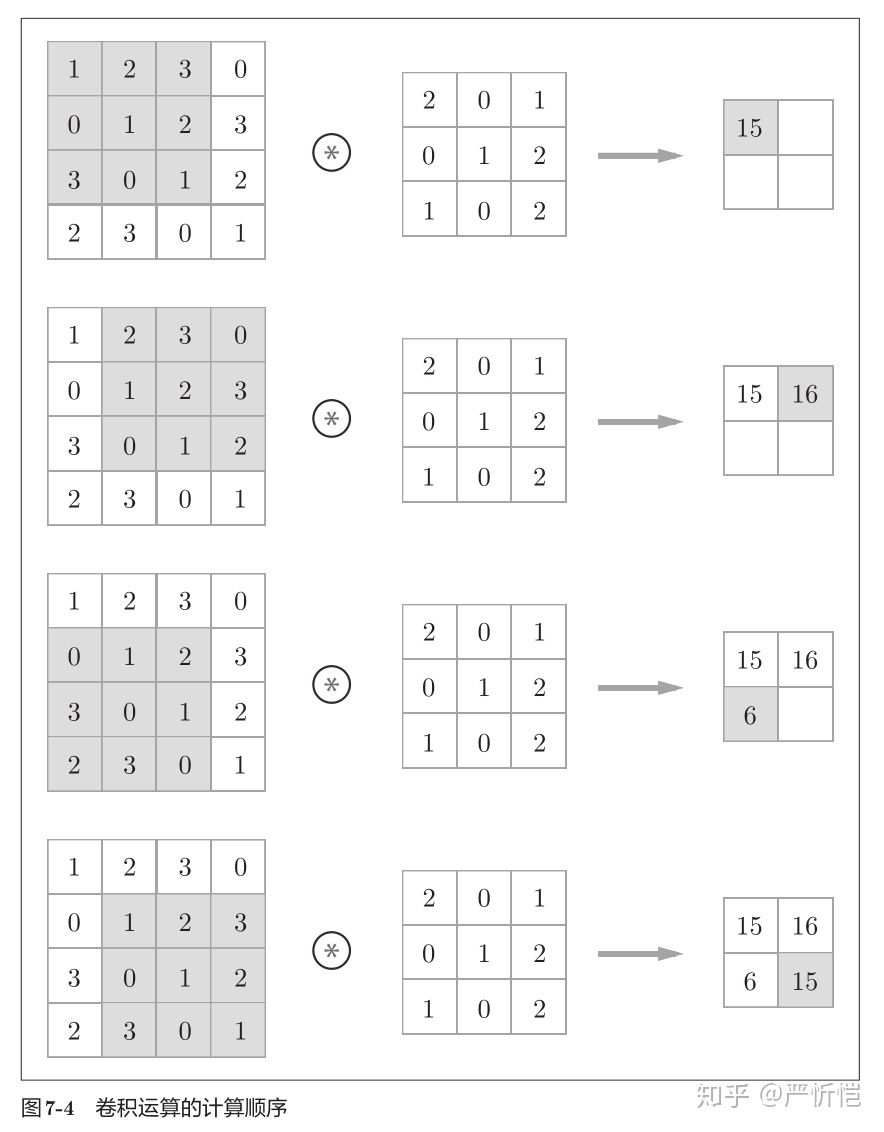
\includegraphics[width=0.90\textwidth]{conv_3}
            \caption{二维离散Valid卷积}
            \label{fig:3}
        \end{figure}
    
        \textbf{Valid卷积} \quad 如图\ref{fig:3}所示,将各个位置上滤波器的元素和输入的对应元素相乘,然后再求和(有时将这个计算称为乘积累加运算)。然后,将这个结果保存到输出的对应位置。将这个过程在所有位置都进行一遍,就可以得到卷积运算的输出。
        
    
        \textbf{Full卷积} \quad 如图所示。
      
        \begin{figure}
            \centering
            \animategraphics[width=\linewidth, autoplay=True, loop=True]{10}{Img/conv_4/conv3-}{0}{35}
            \caption{二维离散Full卷积}
            \label{fig:4}
        \end{figure}
    
        \subsubsection{偏置}
        
        有些时候,在全连接的神经网络中,除了权重参数,还存在偏置。包含偏置的卷积运算的处理流如图\ref{fig:5}所示。
        
        \begin{figure}[!htbp]
            \centering
            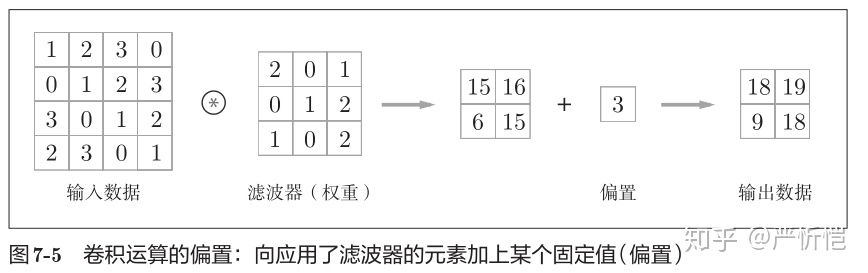
\includegraphics[width=0.90\textwidth]{conv_5}
            \caption{卷积运算中的偏置}
            \label{fig:5}
        \end{figure}
    
        \subsubsection{填充(Padding)}
        
        在进行卷积层的处理之前,有时要向输入数据的周围填入固定的数据(比如0等),这称为填充,是卷积运算中经常会用到的处理。如图\ref{fig:6}所示。
        
        \begin{figure}[!htbp]
            \centering
            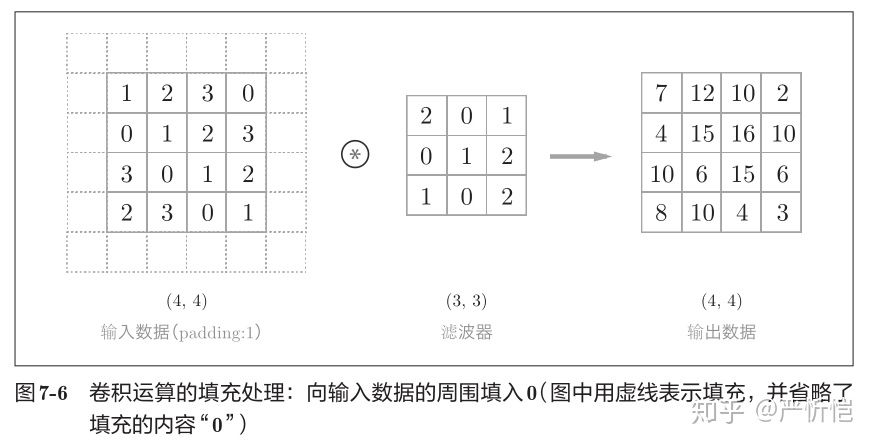
\includegraphics[width=0.90\textwidth]{conv_6}
            \caption{卷积运算中的填充}
            \label{fig:6}
        \end{figure}
    
        从图中可以看出,通过填充,大小为$(4, 4)$的输入数据变成了$(6, 6)$的形状。然后,应用大小为$(3, 3)$的滤波器,生成了大小为$(4, 4)$的输出数据。
        
        使用填充主要是为了调整输出的大小。比如,对大小为$(4, 4)$的输入数据应用$(3, 3)$的滤波器时,输出大小变为$(2, 2)$,相当于输出大小比输入大小缩小了2个元素。如果每次进行卷积运算都会缩小空间,那么在某个时刻输出大小就有可能变为1,导致无法再应用卷积运算。为了避免出现这样的情况,就要使用填充。
        
        \subsubsection{步幅(stride)}
        
        应用滤波器的位置间隔称为步幅(stride)。之前的例子中步幅都是1,如果将步幅设为2,则如图\ref{fig:7}所示,应用滤波器的窗口的间隔变为2个元素。
        
        \begin{figure}[!htbp]
            \centering
            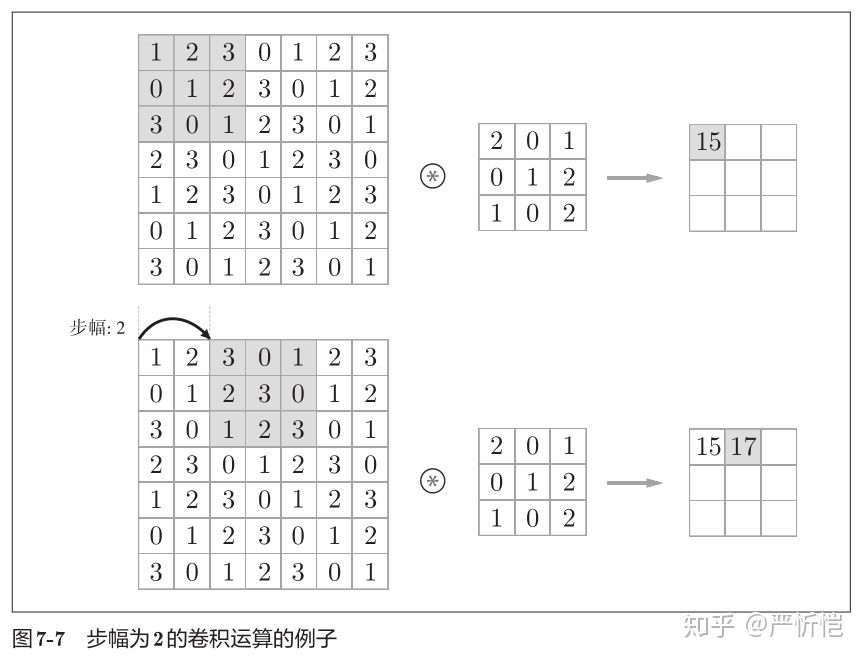
\includegraphics[width=0.90\textwidth]{conv_7}
            \caption{步幅为2的卷积运算}
            \label{fig:7}
        \end{figure}
    
        如图,对输入大小为$(7, 7)$的数据,以步幅2应用了滤波器。通过将步幅设为2,输出大小变为$(3, 3)$。
        
        综上,\uwave{增大步幅后,输出大小会变小。而增大填充后,输出大小会变大}。
        
        \subsubsection{输出大小计算公式}
        
        假设输入大小为$(H, W)$,滤波器大小为$(FH, FW)$,输出大小为$(OH, OW)$,填充为$P$,步幅为$S$。此时,输出大小可通过式\ref{eq:4}进行计算。
        
        \begin{equation}
            \begin{aligned}
                OH &={ {H + 2P - FH} \over {S}} + 1 \\
                OW &={ {W + 2P - FW} \over {S}} + 1
            \end{aligned}
            \label{eq:4}
        \end{equation}

    \subsection{三维数据的卷积运算}   
        
        之前的卷积运算的例子都是以有高、长方向的2维形状为对象的。但是,图像是3维数据,除了高、长方向之外,还需要处理\textbf{通道方向}。
        
        需要注意的是,在3维数据的卷积运算中,输入数据和滤波器的通道数要设为相同的值。其计算方法如图\ref{fig:8}所示。 
        
        \begin{figure}[!htbp]
            \centering
            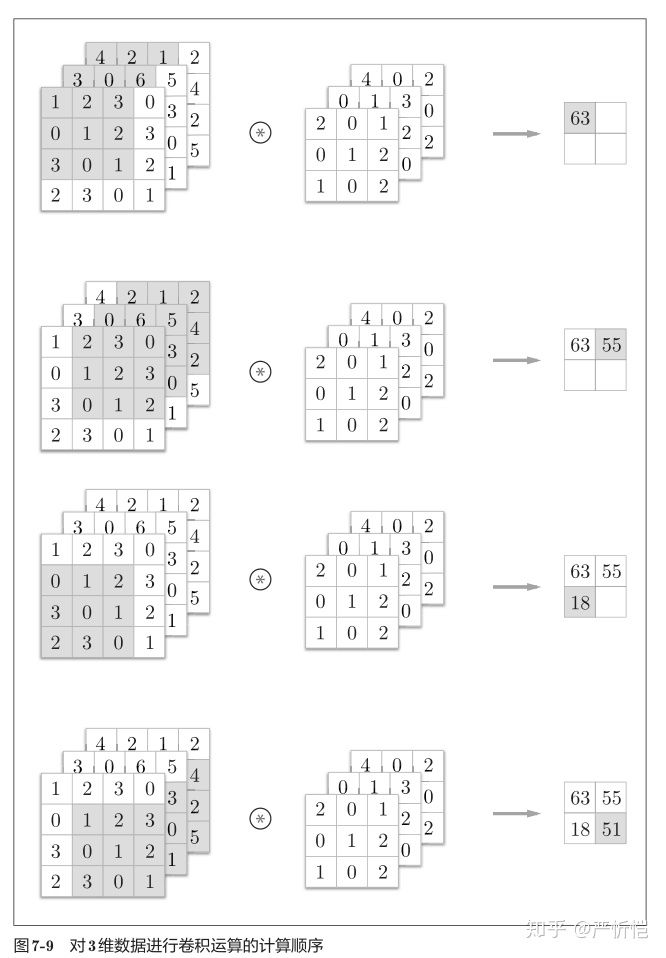
\includegraphics[width=0.90\textwidth]{conv_8}
            \caption{三维卷积运算}
            \label{fig:8}
        \end{figure}
    
        通道方向上有多个特征图时,会按通道进行输入数据和滤波器的卷积运算,并将结果相加,从而得到输出。
        
        将数据和滤波器结合长方体的方块来考虑,3维数据的卷积运算会很容易理解。方块是如图\ref{fig:9}所示的3维长方体。把3维数据表示为多维数组时,书写顺序为$(channel, height, width)$。
        
        \begin{figure}[!htbp]
            \centering
            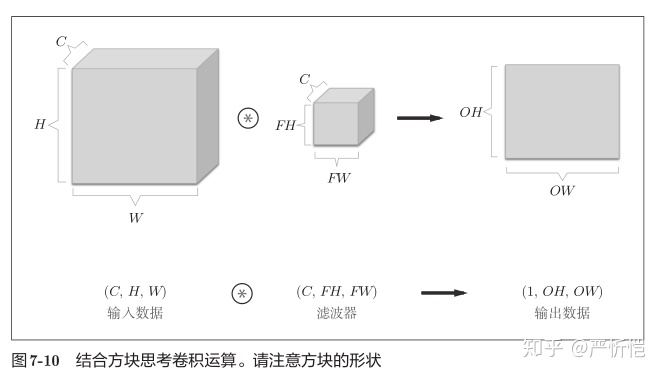
\includegraphics[width=0.90\textwidth]{conv_9}
            \caption{用方块理解三维卷积}
            \label{fig:9}
        \end{figure}
    
        在这个例子中,数据输出是1张特征图。所谓1张特征图,换句话说,就是通道数为1的特征图。那么,如果要在通道方向上也拥有多个卷积运算的输出,该怎么做呢?为此,就需要用到多个滤波器(权重)。用图表示的话,如图\ref{fig:10}所示。
        
        \begin{figure}[!htbp]
            \centering
            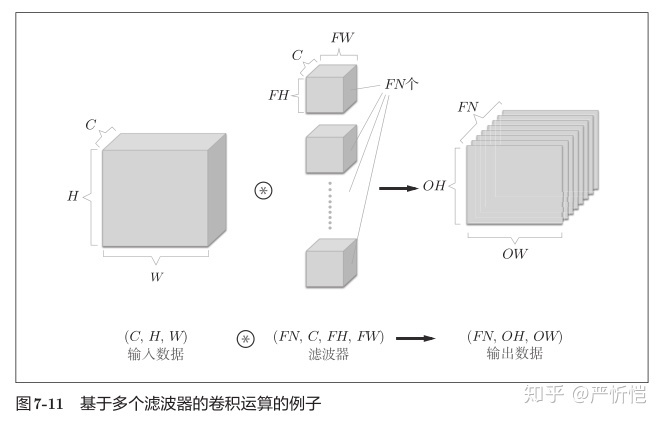
\includegraphics[width=0.90\textwidth]{conv_10}
            \caption{基于多个滤波器的卷积运算}
            \label{fig:10}
        \end{figure}
        
        通过应用FN个滤波器,输出特征图也生成了FN个。如果将这FN个特征图汇集在一起,就得到了形状为$(FN, OH, OW)$的方块。将这个方块传给下一层,就是CNN的处理流。
        
        卷积运算中(和全连接层一样)存在偏置。每个通道只有一个偏置。这里,偏置的形状是$(FN, 1, 1)$,滤波器的输出结果的形状是$(FN, OH, OW)$。这两个方块相加时,要对滤波器的输出结果$(FN, OH, OW)$按通道加上相同的偏置值。
        
            
%---------------------------------------------------------------------------%
% main content
%-
%-> Appendix
%-
%\cleardoublepage%
%\appendix% initialize the environment
%\chapter{中国科学院大学学位论文撰写要求}

学位论文是研究生科研工作成果的集中体现,是评判学位申请者学术水平、授予其学位的主要依据,是科研领域重要的文献资料。根据《科学技术报告、学位论文和学术论文的编写格式》(GB/T 7713-1987)、《学位论文编写规则》(GB/T 7713.1-2006)和《文后参考文献著录规则》(GB7714—87)等国家有关标准,结合中国科学院大学(以下简称“国科大”)的实际情况,特制订本规定。

\section{论文无附录者无需附录部分}

\section{测试公式编号 \texorpdfstring{$\Lambda,\lambda,\theta,\bar{\Lambda},\sqrt{S_{NN}}$}{$\textLambda,\textlambda,\texttheta,\bar{\textLambda},\sqrt{S_{NN}}$}} \label{sec:testmath}

\begin{equation} \label{eq:appedns}
    \adddotsbeforeeqnnum%
    \begin{cases}
        \frac{\partial \rho}{\partial t} + \nabla\cdot(\rho\Vector{V}) = 0\\
        \frac{\partial (\rho\Vector{V})}{\partial t} + \nabla\cdot(\rho\Vector{V}\Vector{V}) = \nabla\cdot\Tensor{\sigma}\\
        \frac{\partial (\rho E)}{\partial t} + \nabla\cdot(\rho E\Vector{V}) = \nabla\cdot(k\nabla T) + \nabla\cdot(\Tensor{\sigma}\cdot\Vector{V})
    \end{cases}
\end{equation}
\begin{equation}
    \adddotsbeforeeqnnum%
    \frac{\partial }{\partial t}\int\limits_{\Omega} u \, \mathrm{d}\Omega + \int\limits_{S} \unitVector{n}\cdot(u\Vector{V}) \, \mathrm{d}S = \dot{\phi}
\end{equation}
\[
    \begin{split}
        \mathcal{L} \{f\}(s) &= \int _{0^{-}}^{\infty} f(t) e^{-st} \, \mathrm{d}t, \ 
        \mathscr{L} \{f\}(s) = \int _{0^{-}}^{\infty} f(t) e^{-st} \, \mathrm{d}t\\
        \mathcal{F} {\bigl (} f(x+x_{0}) {\bigr )} &= \mathcal{F} {\bigl (} f(x) {\bigr )} e^{2\pi i\xi x_{0}}, \ 
        \mathscr{F} {\bigl (} f(x+x_{0}) {\bigr )} = \mathscr{F} {\bigl (} f(x) {\bigr )} e^{2\pi i\xi x_{0}}
    \end{split}
\]

mathtext: $A,F,L,2,3,5,\sigma$, mathnormal: $A,F,L,2,3,5,\sigma$, mathrm: $\mathrm{A,F,L,2,3,5,\sigma}$.

mathbf: $\mathbf{A,F,L,2,3,5,\sigma}$, mathit: $\mathit{A,F,L,2,3,5,\sigma}$, mathsf: $\mathsf{A,F,L,2,3,5,\sigma}$.

mathtt: $\mathtt{A,F,L,2,3,5,\sigma}$, mathfrak: $\mathfrak{A,F,L,2,3,5,\sigma}$, mathbb: $\mathbb{A,F,L,2,3,5,\sigma}$.

mathcal: $\mathcal{A,F,L,2,3,5,\sigma}$, mathscr: $\mathscr{A,F,L,2,3,5,\sigma}$, boldsymbol: $\boldsymbol{A,F,L,2,3,5,\sigma}$.

vector: $\Vector{\sigma, T, a, F, n}$, unitvector: $\unitVector{\sigma, T, a, F, n}$

matrix: $\Matrix{\sigma, T, a, F, n}$, unitmatrix: $\unitMatrix{\sigma, T, a, F, n}$

tensor: $\Tensor{\sigma, T, a, F, n}$, unittensor: $\unitTensor{\sigma, T, a, F, n}$ 

\section{测试生僻字}

霜蟾盥薇曜灵霜颸妙鬘虚霩淩澌菀枯菡萏泬寥窅冥毰毸濩落霅霅便嬛岧峣瀺灂姽婳愔嫕飒纚棽俪緸冤莩甲摛藻卮言倥侗椒觞期颐夜阑彬蔚倥偬澄廓簪缨陟遐迤逦缥缃鹣鲽憯懔闺闼璀错媕婀噌吰澒洞阛闠覼缕玓瓑逡巡諓諓琭琭瀌瀌踽踽叆叇氤氲瓠犀流眄蹀躞赟嬛茕頔璎珞螓首蘅皋惏悷缱绻昶皴皱颟顸愀然菡萏卑陬纯懿犇麤掱暒 墌墍墎墏墐墒墒墓墔墕墖墘墖墚墛坠墝增墠墡墢墣墤墥墦墧墨墩墪樽墬墭堕墯墰墱墲坟墴墵垯墷墸墹墺墙墼墽垦墿壀壁壂壃壄壅壆坛壈壉壊垱壌壍埙壏壐壑壒压壔壕壖壗垒圹垆壛壜壝垄壠壡坜壣壤壥壦壧壨坝塆圭嫶嫷嫸嫹嫺娴嫼嫽嫾婳妫嬁嬂嬃嬄嬅嬆嬇娆嬉嬊娇嬍嬎嬏嬐嬑嬒嬓嬔嬕嬖嬗嬘嫱嬚嬛嬜嬞嬟嬠嫒嬢嬣嬥嬦嬧嬨嬩嫔嬫嬬奶嬬嬮嬯婴嬱嬲嬳嬴嬵嬶嬷婶嬹嬺嬻嬼嬽嬾嬿孀孁孂娘孄孅孆孇孆孈孉孊娈孋孊孍孎孏嫫婿媚嵭嵮嵯嵰嵱嵲嵳嵴嵵嵶嵷嵸嵹嵺嵻嵼嵽嵾嵿嶀嵝嶂嶃崭嶅嶆岖嶈嶉嶊嶋嶌嶍嶎嶏嶐嶑嶒嶓嵚嶕嶖嶘嶙嶚嶛嶜嶝嶞嶟峤嶡峣嶣嶤嶥嶦峄峃嶩嶪嶫嶬嶭崄嶯嶰嶱嶲嶳岙嶵嶶嶷嵘嶹岭嶻屿岳帋巀巁巂巃巄巅巆巇巈巉巊岿巌巍巎巏巐巑峦巓巅巕岩巗巘巙巚帠帡帢帣帤帨帩帪帬帯帰帱帲帴帵帷帹帺帻帼帽帾帿幁幂帏幄幅幆幇幈幉幊幋幌幍幎幏幐幑幒幓幖幙幚幛幜幝幞帜幠幡幢幤幥幦幧幨幩幪幭幮幯幰幱庍庎庑庖庘庛庝庠庡庢庣庤庥庨庩庪庬庮庯庰庱庲庳庴庵庹庺庻庼庽庿廀厕廃厩廅廆廇廋廌廍庼廏廐廑廒廔廕廖廗廘廙廛廜廞庑廤廥廦廧廨廭廮廯廰痈廲廵廸廹廻廼廽廿弁弅弆弇弉弖弙弚弜弝弞弡弢弣弤弨弩弪弫弬弭弮弰弲弪弴弶弸弻弼弽弿彖彗彘彚彛彜彝彞彟彴彵彶彷彸役彺彻彽彾佛徂徃徆徇徉后徍徎徏径徒従徔徕徖徙徚徛徜徝从徟徕御徢徣徤徥徦徧徨复循徫旁徭微徯徰徱徲徳徴徵徶德徸彻徺忁忂惔愔忇忈忉忔忕忖忚忛応忝忞忟忪挣挦挧挨挩挪挫挬挭挮挰掇授掉掊掋掍掎掐掑排掓掔掕挜掚挂掜掝掞掟掠采探掣掤掦措掫掬掭掮掯掰掱掲掳掴掵掶掸掹掺掻掼掽掾掿拣揁揂揃揅揄揆揇揈揉揊揋揌揍揎揑揓揔揕揖揗揘揙揤揥揦揧揨揫捂揰揱揲揳援揵揶揷揸揻揼揾揿搀搁搂搃搄搅搇搈搉搊搋搌搎搏搐搑搒摓摔摕摖摗摙摚摛掼摝摞摠摡斫斩斮斱斲斳斴斵斶斸旪旫旮旯晒晓晔晕晖晗晘晙晛晜晞晟晠晡晰晣晤晥晦晧晪晫晬晭晰晱晲晳晴晵晷晸晹晻晼晽晾晿暀暁暂暃暄暅暆暇晕晖暊暋暌暍暎暏暐暑暒暓暔暕暖暗旸暙暚暛暜暝暞暟暠暡暣暤暥暦暧暨暩暪暬暭暮暯暰昵暲暳暴暵
% appendix content
%-
%-> Backmatter: bibliography, glossary, index
%-
\backmatter% initialize the environment
\intotoc*{\cleardoublepage}{\bibname}% add link to toc
\artxifstreq{\artxbib}{bibtex}{% enable bibtex
    \bibliography{Biblio/ref}% bibliography
}{%
    
    \printbibliography% bibliography
}
%%---------------------------------------------------------------------------%
%->> Backmatter
%---------------------------------------------------------------------------%
\chapter[致谢]{致\quad 谢}\chaptermark{致\quad 谢}% syntax: \chapter[目录]{标题}\chaptermark{页眉}
%\thispagestyle{noheaderstyle}% 如果需要移除当前页的页眉
%\pagestyle{noheaderstyle}% 如果需要移除整章的页眉

感激casthesis作者吴凌云学长,gbt7714-bibtex-style
开发者zepinglee,和ctex众多开发者们。若没有他们的辛勤付出和非凡工作,\LaTeX{}菜鸟的我是无法完成此国科大学位论文\LaTeX{}模板ucasthesis的。在\LaTeX{}中的一点一滴的成长源于开源社区的众多优秀资料和教程,在此对所有\LaTeX{}社区的贡献者表示感谢!

ucasthesis国科大学位论文\LaTeX{}模板的最终成型离不开以霍明虹老师和丁云云老师为代表的国科大学位办公室老师们制定的官方指导文件和众多ucasthesis用户的热心测试和耐心反馈,在此对他们的认真付出表示感谢。特别对国科大的赵永明同学的众多有效反馈意见和建议表示感谢,对国科大本科部的陆晴老师和本科部学位办的丁云云老师的细致审核和建议表示感谢。谢谢大家的共同努力和支持,让ucasthesis为国科大学子使用\LaTeX{}撰写学位论文提供便利和高效这一目标成为可能。

\chapter{作者简历及攻读学位期间发表的学术论文与研究成果}

\textbf{本科生无需此部分}。

\section*{作者简历:}

\subsection*{casthesis作者}

吴凌云,福建省屏南县人,中国科学院数学与系统科学研究院博士研究生。

\subsection*{ucasthesis作者}

莫晃锐,湖南省湘潭县人,中国科学院力学研究所硕士研究生。

\section*{已发表(或正式接受)的学术论文:}

{
\setlist[enumerate]{}% restore default behavior
\begin{enumerate}[nosep]
    \item ucasthesis: A LaTeX Thesis Template for the University of Chinese Academy of Sciences, 2014.
\end{enumerate}
}

\section*{申请或已获得的专利:}

(无专利时此项不必列出)

\section*{参加的研究项目及获奖情况:}

可以随意添加新的条目或是结构。

\cleardoublepage[plain]% 让文档总是结束于偶数页,可根据需要设定页眉页脚样式,如 [noheaderstyle]
%---------------------------------------------------------------------------%
% other information
\end{document}
%---------------------------------------------------------------------------%

